Richiamo di alcuni punti chiave sul piede piatto:

\begin{itemize}
\item
  Il \emph{problema} del piede piatto è essenzialmente di \emph{tipo} \emph{funzionale} e non tanto di tipo estetico e morfologico
\item
  Il piede è una struttura complessa che però alterna dei movimenti semplici: \emph{pronazione e supinazione.}
\item
  Il piede piatto è fondamentalmente una \emph{persistenza di assetto in pronazione} (al contrario il piede cavo è dato da una persistenza dello stato di supinazione).
\item
  La \emph{mancata alternanza} di movimenti di pronazione e supinazione crea dei problemi di \emph{sovraccarico} e di conseguenza \emph{tutta la sintomatologia} del piede piatto nell'adulto (di qualunque eziologia esso sia) deriva da questo \emph{mancato riposo delle strutture:} la patologia del tibiale posteriore, le fasciti plantari, l'alluce valgo, la tendinopatia.
\item
  Il piede piatto è molto comune in età pediatrica infatti è la seconda (se non prima) causa di consultazione dell'ortopedico in età infantile.
\end{itemize}

\section{Piede piatto, trattamento}

Nel piede piatto l'astragalo si sposta verso il basso e ruota all'interno e con esso anche la gamba.

E' intuitivo che il trattamento sia quello di \textbf{\emph{riposizionare l'astragalo sopra al calcagno}} e di \textbf{\emph{riportare il calcagno in asse con la tibia}}.

\emph{Il problema reale non è la scomparsa della volta plantare} (problema che affligge soprattutto i genitori o chi non conosce la patologia). Basti pensare a certi atleti come Usain Bolt che non ha la volta plantare, ma è palesemente solo un problema di tipo estetico: la realtà è che non ha la volta plantare, ma ha un calcagno dritto per cui nessun deficit funzionale.

Dal punto di vista funzionale quello che conta (e che quindi condizionerà anche il trattamento della patologia) è la \textbf{rotazione esterna del calcagno} ovvero l'eccesso di pronazione.

Il trattamento (in qualunque forma di piede piatto) deve volgere a ricostituire l'anatomia fisiologica quanto più possibile quindi a \emph{riallineare il tallone} (inteso non solo come calcagno, ma come l'intera struttura astragalo-calcaneare) attraverso un \emph{ripristino
dei rapporti astragalo-calcaneari. }

\emph{Il trattamento deve tenere conto delle diverse forme di piede piatto e quindi è necessario fare una corretta e precisa diagnosi, tenendo conto delle diverse possibili eziologie.} Come per la trattazione generale del piede piatto anche per il trattamento,particolare attenzione sarà riservata al trattamento del piede piatto essenziale (quello del bambino) per almeno due ragioni fondamentali:

\begin{itemize}
\item
  E' ampiamente diffuso
\item
  \emph{In età infantile il trattamento del piede piatto nei casi di \textbf{deficit funzionale è essenziale} per prevenire un'evoluzione in senso degenerativo che nell'adulto richiederebbe un trattamento chirurgico molto più complesso ed invasivo.}
\end{itemize}

\textbf{\emph{N.B. il trattamento del piede piatto trova indicazione solo se c'è un deficit funzionale}}

\begin{figure}[!ht]
\centering
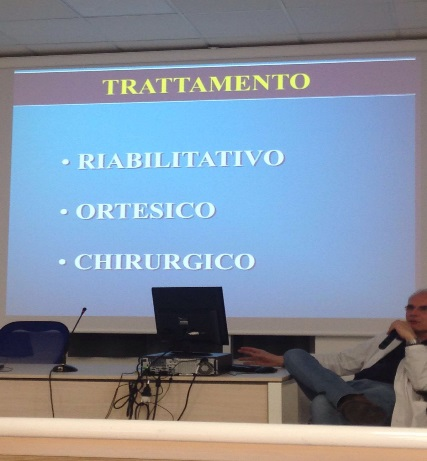
\includegraphics[width=0.4\textwidth]{015/image1.jpeg}
\end{figure}

Il trattamento di questa deformità può essere di 3 tipi:
\begin{itemize}
\item[1.] Ortesico
\item[2.] Riabilitativo
\item[3.] Chirurgico
\end{itemize}

{[}Il consumo della suola delle scarpe all'esterno non è indice di problematiche nella deambulazione o della presenza di piede piatto. Anzi è qualcosa di fisiologico perché l'appoggio del piede inizia con il bordo esterno (perché si va in supinazione), quindi è ovvio che quando
si appoggia la scarpa a terra essa poggia prima nella parte esterna.{]}

\subsection{Il trattamento Ortesico}

\begin{figure}[!ht]
\centering
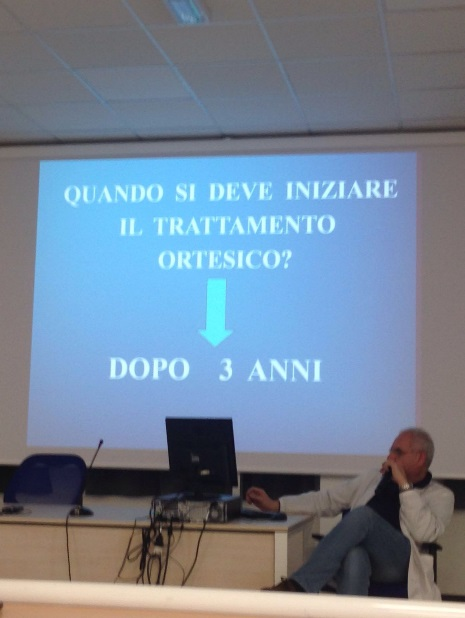
\includegraphics[width=0.4\textwidth]{015/image2.jpeg}
\end{figure}


Fino ai 3-4 anni il piede piatto è \emph{fisiologico} per cui è inutile utilizzare dei plantari prima di quell'età a meno che non si abbia il caso di un piede piatto con astragalo verticale estremamente severo.

\begin{itemize}
\item
  Non esiste il piede piatto prima dei 4 anni
\item
  \emph{Non è assolutamente valido il concetto di plantare preventivo}
\end{itemize}

Nei primi anni di vita quando il piede piatto è fisiologico, sarà l'alternanza di pronazione e supinazione (quando il bambino comincia a camminare) e gli stimoli legati alla deambulazione che faranno sì che il piede abbia un suo normale sviluppo morfologico.

\begin{figure}[!ht]
\centering
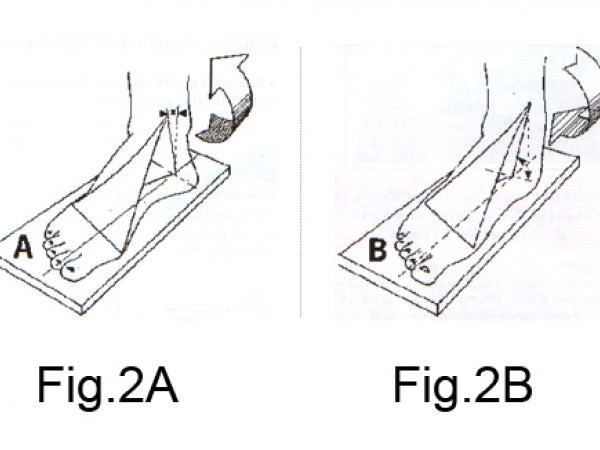
\includegraphics[width=0.4\textwidth]{015/image3.jpeg}
\end{figure}


Quando camminiamo il piede ha una torsione che ricorda il doppio giro dell'elica di un aereo (vedi Figc. 2A e 2B). Nel piede piatto questa torsione è esasperata.

Dopo i 4 anni possiamo parlare propriamente di piede piatto e da questa età e fino agli 8 anni il trattamento sarà \textbf{ORTESICO} (si parla di età scheletrica non anagrafica) ovvero con \textbf{plantari.}

Negli anni '80 si pensava che bisognasse ristabilire la volta plantare (\textbf{\emph{errato}}!) e quindi i plantari erano progettati come delle mezzaluna. Però l'apice del plantare cadeva in un punto dove non bisognava spingere!

Quindi si è passati al \textbf{quarto di sfera} che non aveva lo scopo di rimodellare la volta plantare, ma aveva lo scopo di \emph{spingere su l'astragalo}.

Poi vennero creati negli anni 90' plantari in plexiglass che si scoprirono tossici per i materiali usati.

Oggi vengono utilizzati dei plantari \emph{rigidi confezionati su misura} e questi hanno minime controindicazioni come la comparsa di calli.

{[}Il prof sottolinea di non esser mai riuscito a dimostrare che il miglioramento sia effettivamente merito del plantare. {]}

I plantari hanno la funzione di:

\begin{itemize}
\item[1.]
  Correggere la deformazione. Questo sarà possibile perché il plantare permette di:
\begin{itemize}
\item
  Risollevare l'astragalo e riportarlo all'altezza del calcagno così da normalizzare i rapporti reciproci tra tali strutture ossee
\item
  Tenere riallineato il retro-piede in modo tale che l'osso e le parti molli si rimodellino con l'accrescimento: è chiaro che dal momento che il piede è flessibile, una volta riallineato il retro-piede, l'avampiede da solo realizzerà il \emph{movimento ``dell'elica''} e questo permetterà di ottenere una normalizzazione di tutte le ossa della parte media e anteriore del piede.
\end{itemize}
\item[2.]
  Contenere la correzione
\item
  Indirizzare l'accrescimento (vedi punto 1)
\end{itemize}

Il plantare va portato a tempo pieno (il più possibile) \emph{e mantenuto per un tempo sufficientemente lungo da permettere la ristrutturazione delle ossa e il ritensionamento delle strutture molli mediali del piede (in genere 4 anni)}

Se il bambino con il plantare gioca, corre e fa una vita normale, questi stessi movimenti fungeranno da riabilitazione fatta su un piede che \emph{è obbligato dal plantare a mantenere una certa posizione}: il rimodellamento osseo in questa fase di accrescimento potrà contribuire alla correzione. Tale correzione però non dovrà esser valutata sulla base della morfologia della volta plantare, ma in termini di ripristino funzionale.

Se infatti la morfologia non è valida al momento della diagnosi, non lo sarà neanche al termine del trattamento e non potrò nemmeno giudicare la correzione sulla base di questa (anche l'intervento chirurgico molte volte non ristabilisce la volta plantare anche perché il fine è di
riallineare il tallone così da permettere il recupero funzionale piuttosto che ripristinare la volta plantare).

\emph{Quindi la morfologia non va bene né per la diagnosi né per valutare i risultati}.

\begin{figure}[!ht]
\centering
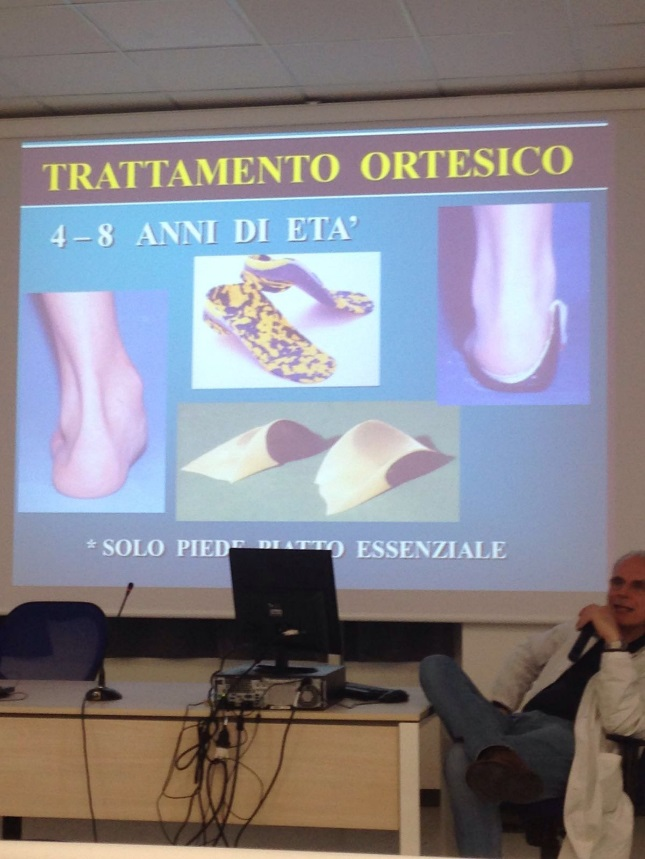
\includegraphics[width=0.4\textwidth]{015/image4.jpeg}
\end{figure}


{[}Bisogna spiegare alle mamme che non si ridà un ``piede normale'' dal loro punto di vista ovvero con la volta plantare, ma dal punto di vista medico cioè funzionale{]}.

Ci sono casi in cui il \textbf{plantare non va utilizzato}:

\begin{itemize}
\item
  Piede con ``barra'': se il piede è rigido con una barra non sarà possibile alcuna correzione
\item
  Retrazione del tendine d'Achille che impedisce il fenomeno di inversione dell'elica.
\end{itemize}

\textbf{\emph{Solo il piede piatto essenziale è trattato con i plantari}} perché le altre forme di piede piatto non si giovano dell'utilizzo di questo.

\subsection{Il trattamento riabilitativo}

Si possono associare esercizi fisioterapici al trattamento con plantare oltre alla normale attività sportiva.

\emph{Il trattamento fisioterapico viene associato a quello ortesico attraverso la prescrizione di esercizi mirati al potenziamento dei cosiddetti ``\textbf{muscoli cavizzanti}'' che consistono in esercizi di pressione di oggetti (matite o fazzoletti) o di deambulazione guidata
sulla punta dei piedi o sul bordo esterno.}

\begin{figure}[!ht]
\centering
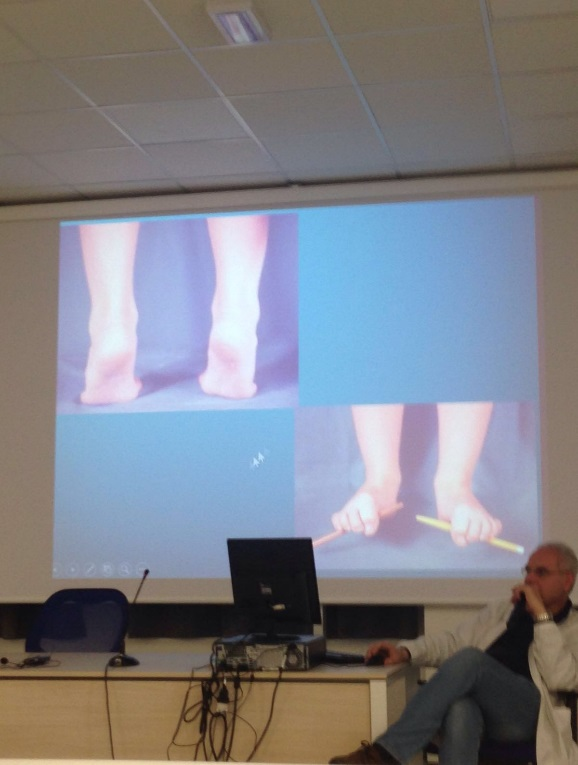
\includegraphics[width=0.4\textwidth]{015/image5.jpeg}
\end{figure}


E' estremamente importante non limitare in alcun modo le attività del bambino (correre, giocare, saltare, ecc.) che rappresenta la migliore fisioterapia dal momento che con i plantari permettono di ripristinare i rapporti astragalo-calcaneari.

Il plantare si abbandona:

\begin{itemize}
\item
  Quando la \emph{deformità è corretta}, anche se questo è più un discorso di tipo morfologico che funzionale.
\item
  \emph{Dopo gli 8 anni di età} quando è inutile portare un plantare e si può passare ad un trattamento chirurgico. Dopo gli 8-10 anni d'età se il piede è ancora funzionalmente piatto, iniziano i disturbi. Quindi se si mantiene il plantare oltre gli 8 anni, non farà nulla dal punto di vista correttivo, ma maschererà un sintomo che è il discomfort e questo toglie una possibile indicazione al trattamento chirurgico. \textbf{\emph{Dopo gli otto anni va assolutamente abbandonato!}}
\item
  Dopo 3 anni di trattamento senza risultato
\end{itemize}

\subsection{Il trattamento chirurgico}

Il trattamento chirurgico è limitato al 15\% dei casi. Le indicazioni per il trattamento chirurgico sono:

\begin{itemize}
\item
  Piede piatto essenziale dopo gli otto anni perché si è visto che se il bambino viene operato prima degli 8 anni, la protesi non tiene. Invece dagli 8 anni in poi il trattamento è efficace
\item
  Piede piatto sintomatico
\item
  \textbf{Insufficienza funzionale} con dolore anche alle ginocchia: dolore un po' ovunque e questo vuol dire che il piede è in uno stato di persistente pronazione ed è necessario l'intervento chirurgico
\end{itemize}

Per il trattamento chirurgico occorre che il piede si sia già sviluppato, ma \textbf{\emph{che abbia ancora del potenziale d'accrescimento per questo è indicato dopo gli otto anni.}}

\begin{figure}[!ht]
\centering
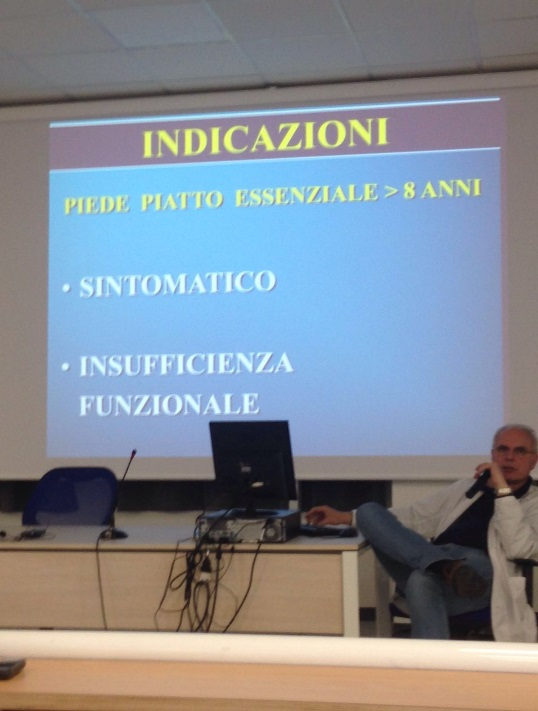
\includegraphics[width=0.4\textwidth]{015/image6.jpeg}
\end{figure}

L'intervento chirurgico ha lo stesso scopo di quello del plantare solo che lo si fa da dentro tanto è vero che è denominato ENDOORTESI.

L'intervento si chiama \textbf{ARTRORISI SOTTOASTRAGALICA} perché la sottoastragalica viene limitata nel suo movimento di pronazione. \emph{Limitando l'escursione articolare del calcagno in rotazione esterna (cioè in pronazione), si agisce sulla causa prima dello scivolamento dell'astragalo in basso e medialmente.} \emph{Questa artrorisi prevede l'uso di viti o piccole protesi che vengono posizionate a livello del seno del tarso} (una zona tra astragalo e calcagno) \emph{tramite una piccola incisione fra astragalo e calcagno, senza ledere le struttura anatomiche del piede.} La rotazione del calcagno è limitata perché viene impiegato un cilindretto simile ad una vite ad espansione che permette sia di mantenere i rapporti tra astragalo e calcagno sia di evitare che in stazione eretta il piede crolli in pronazione (cioè in rotazione esterna del calcagno).

Di solito in età di accrescimento l'endortesi è \emph{l'unica} procedura eseguita.

L'impianto dava il 94\% di buoni risultati, l'unico problema era la rimozione e quindi negli anni 90', con l'avvento dei materiali riassorbibili, si studiarono nuove protesi con materiali come l'\textbf{acido poli-L-lattico}.

Il materiale riassorbibile, grazie alla vascolarizzazione locale, viene a poco a poco degradato.

\begin{figure}[!ht]
\centering
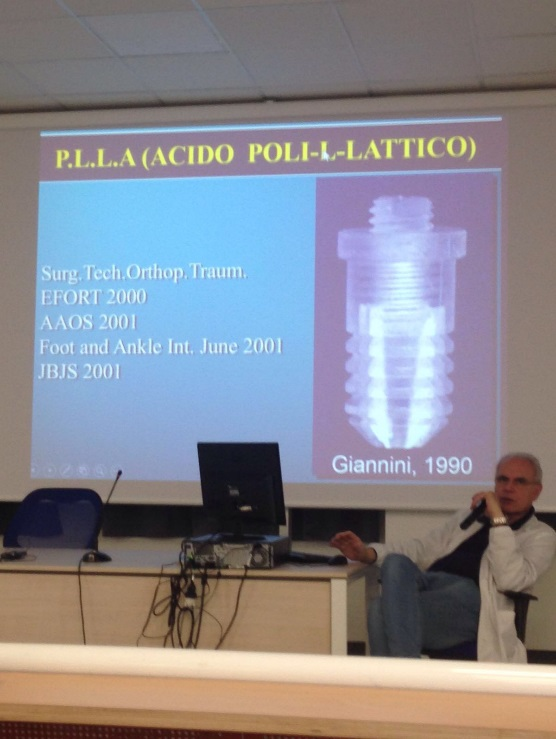
\includegraphics[width=0.4\textwidth]{015/image7.jpeg}
\end{figure}

La tenuta meccanica è di circa 2 anni e mezzo, mentre in 5 anni viene completamente riassorbito.

\begin{figure}[!ht]
\centering
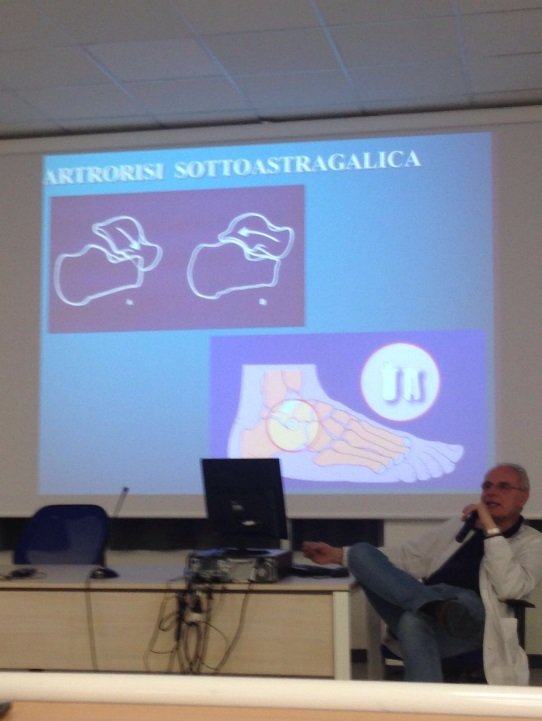
\includegraphics[width=0.4\textwidth]{015/image8.jpeg}
\end{figure}

\begin{figure}[!ht]
\centering
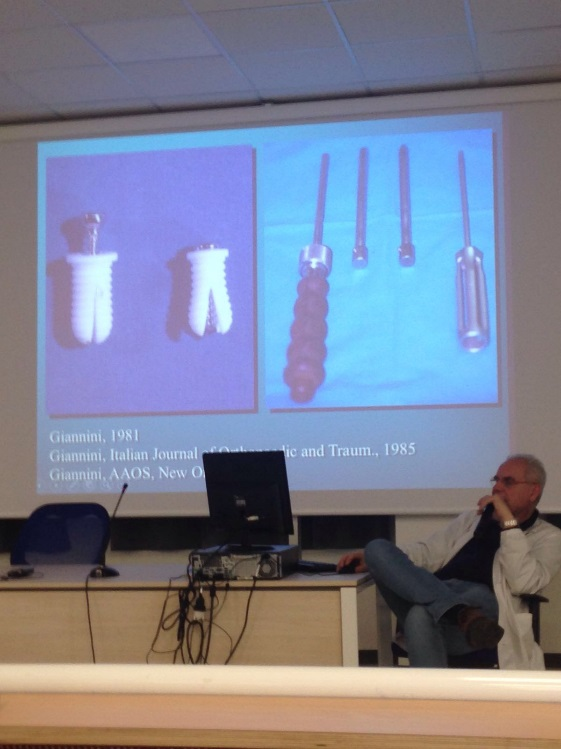
\includegraphics[width=0.4\textwidth]{015/image9.jpeg}
\end{figure}


Ci sono però dei \textbf{trattamenti chirurgici accessori} che vanno eseguiti in certe condizioni

Questi sono:

\begin{itemize}
\item
  \emph{L'allungamento tendine d'Achille}. È un intervento molto difficile e si esegue in percutaneo.

Si introduce una lametta da 15 e si fanno delle emisezioni ad entrambi i lati del tendine (bisogna stare attenti a non tagliare tutto il tendine) così da indebolirlo. Quindi successivamente il piede viene stressato in flessione dorsale così da allungare il tendine che si sfibra senza però causarne l'interruzione. \emph{Questa procedura trova indicazione quando il piede non raggiunge l'angolo retto dopo l'artrorisi.}

\item
  \emph{Il tempo mediale di ritenzione del tibiale posteriore.} Abbiamo parlato di \emph{scafoide accessorio} e \emph{scafoide prominente} cioè quella parte di osso che sporge dalla parte interna e che può causare dolente ad esempio se si strofina con la scarpa. In realtà però essendo proprio nella zona dove si inserisce il tibiale posteriore, può essere anche la causa di una \emph{insufficienza funzionale} di questo tendine che sarà più lungo dal momento che c'è un osso in più. Quando è presente, sarà necessario rimuovere questo scafoide accessorio, staccare il tendine e re-inserirlo.
\end{itemize}

Quando si eseguono questi tempi chirurgici accessori c'è un tempo di immobilizzazione in gesso che è più lungo arrivando fino a 6 settimane: le prime 4 non si cammina.

In caso di sola endortesi dopo 3 settimane si può camminare mentre se si fanno uno o entrambi dei tempi accessori, è necessario uno stivaletto gessato per 6 settimane. Di queste, 3-4 settimane senza carico e poi si cammina altre due settimane sempre mantenendo lo stivaletto.

In tutti i casi comunque quello che conta è l'allineamento del retropiede.

Questo intervento ha anche \emph{altre indicazioni} oltre a quelle del piede piatto essenziale:
\begin{itemize}
\item \emph{l'Astragalo verticale} detto anche piede a dondolo,
\item Il cosiddetto \emph{piede ad equino}. In questo caso non basta solo l'endortesi, ma questa viene eseguita lo stesso per aiutare a mantenere i rapporti tra astragalo e calcagno.
\item Il \emph{piede piatto sinostosico} cioè dovuto ad una mancata segmentazione tra astragalo e calcagno o tra calcagno e scafoide.
L'ortesi può essere fatta previa eliminazione della barra. Una volta tolta la barra ovvero il ponte osseo, allora si può posiziona l'endortesi.
\end{itemize}

L'insufficienza funzionale da piede piatto nell'adulto con il tempo porta ad \textbf{alluce valgo}.

Se il piede piatto non dovesse esser curato in età infantile, è possibile un intervento anche nell'adulto però non si può sperare in un grosso rimodellamento che tra l'altro avverrà in tempi più lunghi.

Quindi questo intervento può essere fatto anche nell'adulto purché il piede sia elastico.

In questo caaso non è pensabile eseguire solo l'endortesi, ma bisogna sempre fare l'allungamento del tendine d'Achille e un intervento di ritenzione del tibiale posteriore.

Se il piede è \emph{artrosico o rigido} l'intervento non può essere eseguito.

\subsection{Le controindicazioni}

Lo scopo di questa protesi è quello di mantenere i rapporti tra astragalo e calcagno per un tempo sufficientemente lungo affinché le ossa si possano ristrutturare. Si pensa che nel \textbf{\emph{piede piatto neurologico}}, prevalentemente nel flaccido (poliomielite), questo non possa avvenire, mentre nello spastico sì:

\begin{itemize}
\item
  Piede piatto neurologico tipo \textbf{flaccido} è una \textbf{controindicazione assoluta all'intervento}
\item
  Piede piatto neurologico tipo \textbf{spastic}o è una \textbf{controindicazione relativa} In questo caso si può anche utilizzare la protesi, ma bisogna stare molto più attenti al tibiale posteriore e nel fare l'allungamento del tendine d'Achille.
\end{itemize}

In generale si dice che nel piede piatto neurologico questo intervento è controindicato. Allora si fa un intervento simile, ovvero una \textbf{ARTRODESI} dove si bloccano i rapporti tra astragalo e calcagno in correzione.

L'artrodesi è effettuata nello stesso punto dove viene messa l'ortesi: mentre l'ortesi mantiene il movimento tra astragalo e calcagno perché l'articolazione non l'abbiamo toccata, l'artrodesi blocca l'articolazione attraverso l'utilizzo di un \emph{pezzetto d'osso prelevato dall'epifisi prossimale} della stessa tibia.

Questo intervento è proprio nato per i piedi spastici, inventato da un certo Grays.

Ovviamente questi piedi piatti sono molto più gravi rispetto a quello idiopatico del bambino.

Altra controindicazione è la \textbf{\emph{lassità legamentosa grave}} dove si perde sia la funzione che la morfologia. Si tratta di deformità importanti e anche in questo caso si può eseguire un'artrodesi.

Molto spesso il piede piatto è pronato non perché ci sia un'anatomia sovvertita tra astragalo e calcagno, ma perché c'è un valgo a livello della caviglia quindi si fanno altre cose come un riallineamento del retropiede attraverso un'osteotomia del calcagno.
